
\chapter{Formulations in linear elasticity}
\section{Strong formulation}	
	The equilibrium equations omitting concentrated body moments and the material law in linear elasticity for isotropic and homogeneous materials are:
	
	\begin{equation}
	b_i + \tau _{ij,j} = 0, \qquad \epsilon _{ij} = \frac{1}{E }[(1+\nu) \tau _{ij} - \nu \delta _{ij} \tau _{kk}].
	\end{equation}
	
	Since there is a linear relation between stresses and strains, strain tensor $\epsilon _{ij}$ derives itself from the displacement field, we can rewrite the equilibrium equations in function of the displacements. This leads to the \textbf{displacement-based finite element method}, the unknowns are the displacements. All the set of equations are encompassed under the \textbf{strong formulation} therminology, because they require to be satisfied \textbf{locally}, at each point of the domain V.
	
\subsection{Boundary conditions}
	The main classes of boundary conditions are: 
	
	\begin{itemize}
	\item[•] \textbf{essential boundary conditions} (Dirichlet): the displacement is prescribed on a portion of the external surface $S$, called $S_u$; \\
	
	\item[•] \textbf{natural boundary conditions} (Neumann): the contact force is imposed on another portion of the external surface $S$, called $S_t$. 
	\end{itemize}
	
\subsection{Mathematical properties of the governing equations}
	First, the \textbf{superposition principle} is respected by stresses, strains and displacements because linearity of the static and kinematic equations in linear elasticity (assuming small displacements/strains). Indeed if $\tau _{ij}^A$ and $\tau _{ij}^B$ are stress tensors associated to load cases A and B, $\tau _{ij}^A + \tau _{ij}^B$ is the solution for the load case A + B. \\
	
	Secondly, for given surface and body forces, the uniqueness of the solution for the governing equations is guaranteed. 
	
	\proof{\ \\
		
	As a counterargument, let's assume that there exist two solution $u_i^{(1)}$ and $u_i^{(2)}$ and their difference $u_i ' = u_i^{(1)}-u_i^{(2)}$. Let's do the same for strains and stresses:
	
	\begin{equation}
	\epsilon _{ij} ' = \epsilon_{ij}^{(1)}-\epsilon _{ij}^{(2)}, \qquad \tau _{ij} ' = \tau _{ij}^{(1)}-\tau _{ij}^{(2)}.
	\end{equation}
	
	Since the body forces are external and identical for the two solutions, we get from the equilibrium equations:
	
	\begin{equation}
	\epsilon_{ij,j}^{(1)}-\epsilon _{ij,j}^{(2)} = \epsilon _{ij,j} ' = 0. 
	\end{equation}
	
	On the other hand, the strain energy of the difference is:
	
	\begin{equation}
	W' = \frac{1}{2}\int _V \epsilon _{ij} ' \tau _{ij} ' \, dV =  \frac{1}{2}\int _V \frac{1}{2} (u _{i,j} '+ u _{j,i} ') \tau _{ij} ' \, dV = \frac{1}{2}\int _V u' _{i,j} \tau _{ij} ' \, dV,
	\end{equation}
	
	by symmetry and as i, j are repeated. If we use integration by part and Gauss theorem, we get:
	
	\begin{equation}
	\begin{aligned}
	W' &= \frac{1}{2} \int _V (u' _{i} \tau ' _{ij})_{,j} \, dV - \frac{1}{2} \cancel{\int _V u' _{i} \tau ' _{ij,j} \, dV} \\
	&= \frac{1}{2} \oint _S u' _{i} \tau ' _{ij} n_j \, dV = \frac{1}{2} \oint _S u' _{i} \bar{\tau '} _{i}^{(n)} \, dV
	\end{aligned}
	\end{equation}
	
	To guarantee the uniqueness of the solution, so to have $W' = 0$, the boundary conditions must satisfy:
	
	\begin{enumerate}
	\item the displacement field $u_i$ is prescribed on the entire surface, leading directly to $u_i ' = 0$
	
	\item the contact forces $t_i ^{(n)}$ are imposed over the entire surface while overall equilibrium is satisfied, making $t_i ^{'(n)} = 0$
	
	\item displacements $u_i$ are prescribed on one part of the surface ($u_i = \bar{u}_i$ on $S_u$), while contact forces $\tau _i^{(n)}$ are imposed on the rest of the surface ($\tau _i^{(n)} = \bar{\tau} _i^{(n)}$ on $S_t$), so that either $u_i '= 0$ or $\tau _i^{(n)}= 0$. The $\bar{ }$ symbol indicates that the values are prescribed. 
	\end{enumerate}
	}
	
	This explains why it is not allowed to impose both the displacement and the force on the same point and the same direction. Example on \autoref{fig:4.1}. 
	
	\begin{center}
	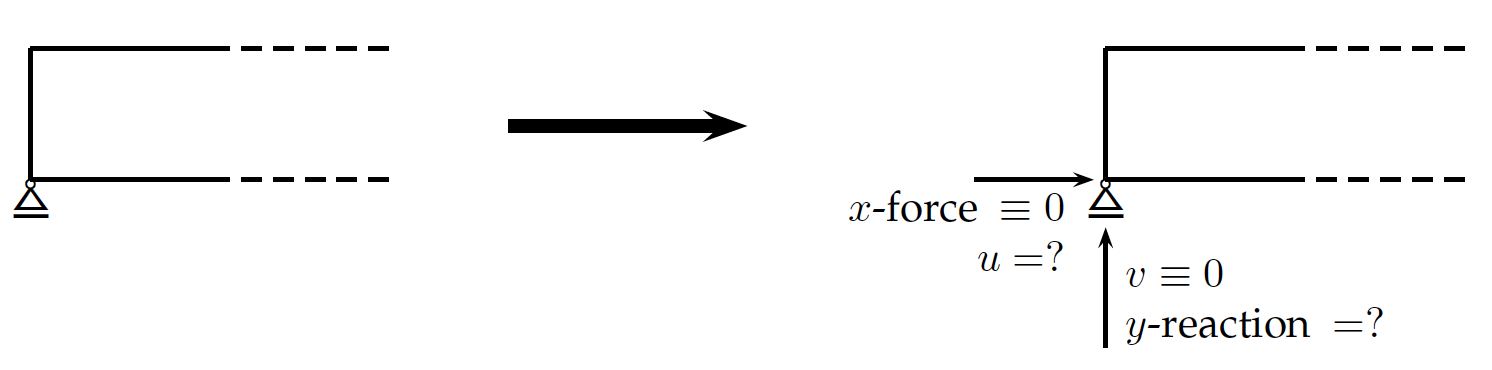
\includegraphics[scale=0.3]{ch4/1}
	\captionof{figure}{}
	\label{fig:4.1}
	\end{center}